%!TEX root = ../main.tex
% Chapter 1

\chapter{Einleitung}
\label{Einleitung}

Dieses Kapitel leitet in die grundlegende Thematik von E-Mails ein. Nach einer Erläuterung dieser Domäne wird das sich daraus ergebende Problemfeld beschrieben und mögliche Folgen dessen skizziert. Die Bearbeitung des Problemfelds ergibt eine Forschungsfrage, die diese Arbeit inhaltlich lenkt. Darüber hinaus wird die Vorgehensweise beschrieben, mit welcher die Forschungsfrage beantwortet werden soll.

\section{Kontext und Domäne}
\label{Kontext_und_Domaene}
Die E-Mail ist in den letzten drei Jahrzehnten zu einem der wichtigsten Kommunikationsmittel aufgestiegen. Diese Entwicklung lässt sich anhand verschiedener Faktoren beobachten.

Grundsätzlich ist die Anzahl der E-Mail Nutzer kontinuierlich gestiegen. Während 2002 nur 38\% der Bevölkerung in Deutschland das Internet für E-Mails nutzten, betrug der Wert im Jahr 2020 87\% \citep{SAEU2022}. Insbesondere in der Altersgruppe von 16 bis 64 Jahren gaben in einer Studie im Jahr 2020 über 90\% der Befragten an in den letzten drei Monaten E-Mails versendet oder empfangen zu haben \citep{StatistischesBundesamt2021}. Diese hohen Nutzerzahlen verdeutlichen die hohe Relevanz, die die E-Mail im alltäglichen Leben hat.

Ein weiterer Indikator ist die Anzahl der versendeten E-Mails, welche von 2000 (32,3 Milliarden) bis 2018 (848,1 Milliarden) um das 26-fache anstieg, Spam-Mails exkludiert \citep{MMG2018}. Auffällig ist insbesondere der Anstieg im Jahr 2017 um 146 Milliarden E-Mails. Dies ist zum Einen durch eine erhöhte Nutzung von natürlichen Personen, aber auch durch eine erhöhte Anzahl an \textit{technischen E-Mails} zu erklären.  \gls{technischeemail}s sind E-Mails, welche von Systemen automatisch versendet werden, zum Beispiel zur Registrierung von Nutzern, Information von Nutzern, Newslettern oder \acrfull{2fa}. Letztere erklärt den Anstieg des E-Mail Verkehrs von 2017, da in diesem Jahr die EU-Verordnung zur verpflichtenden Nutzung von 2FA in beispielsweise Online-Banking eingeführt wurde \citep{EuropaeischeKommission2017}. Dies hat zur Folge, dass bei jedem Login eine SMS, App-Benachrichtigung, E-Mail etc. versendet wird.

E-Mails lassen sich nicht nur anhand ihres Absenders (Mensch/System), sondern auch anhand ihres Zweckes unterscheiden. So sind die Einsatzzwecke vielfältig und umfassend. In einer Studie der \cite{MMG2020} gaben 63\% der Befragten an mit Firmen, 54\% mit Bekannten und Familie, 53\% mit Ämtern, 38\% mit Freunden und 20\% mit Lebenspartnern über E-Mails zu kommunizieren.

Die Nutzung in verschiedenen Kontexten hat zur Folge, dass E-Mails, insofern sie je nach Einsatzzweck nicht strikt in verschiedenen Konten sortiert sind, eine Sichtung benötigen. Eine solche Sichtung, auch \textit{\gls{triage}} genannt, bezeichnet den \emph{\glqq[...] Prozess, bei dem unbearbeitete E-Mails durchgesehen und entschieden wird, was damit zu tun ist.\grqq{}} \citep[S. 325]{Sarrafzadeh2019}. \gls{triage} ist, insbesondere im beruflichen Kontext, relevant für die persönliche Aufgabenverwaltung und die Produktivität. Die aus einer Triage entstehenden Handlungsschritte können die Beantwortung, das Lesen, das Löschen, das Sortieren oder die Archivierung einer E-Mail sein. \cite{Sarrafzadeh2019} identifizieren innerhalb der Triage drei Schritte: Priorisierung, Zurückstellung und Strategien zur Erleichterung der Wiedervorlage. Der Ablauf einer Triage ist als Flussdiagramm in Abbildung \ref{fig:triage_ablauf} dargestellt.

In der Priorisierung versucht der Nutzer die Intention von E-Mails und einen möglichen Handlungsbedarf zu identifizieren. Verschiedene Strategien zur Priorisierung werden im nächsten Absatz näher erläutert. Nachdem E-Mails ohne direkten Handlungsbedarf aussortiert wurden, wird in der Zurückstellung entschieden, welche E-Mails direkt und welche E-Mails vorerst nicht bearbeitet werden. Die Entscheidung über eine Zurückstellung wird insbesondere dadurch entschieden, ob Empfänger zeitnah eine Rückmeldung geben können und ob die E-Mail eine Dringlichkeit aufweist \citep[S. 327]{Sarrafzadeh2019}. Zurückgestellte E-Mails werden zu einem späteren Zeitpunkt beantwortet. Damit Empfänger diese Wiedervorlage als Aufgabe nicht vernachlässigen, werden Strategien zur Erleichterung angewendet. Diese Strategien sind individuell und können beispielsweise die Sortierung von E-Mails in verschiedenen Ordnern, das Markieren mit bestimmten Stichwörtern oder die Erinnerung über ToDo-Listen, Kalender und andere Tools sein.

\begin{figure}[!ht]
	\centering
		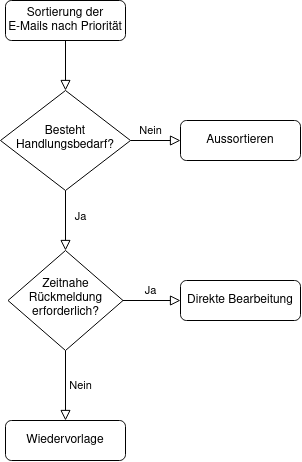
\includegraphics[width=0.5\textwidth]{Figures/Triage.png}
	\caption[Ablauf einer Triage]{Ablauf einer Triage nach \cite{Sarrafzadeh2019}}
	\label{fig:triage_ablauf}
\end{figure}

\noindent Da sowohl die Zurückstellung, als auch die Strategien zur Erleichterung der Wiedervorlage als Folgeaufgabe aus der Priorisierung entstehen, kann dieser eine übergeordnete Rolle zugewiesen werden. Hierbei entscheidend sind die Faktoren, die die Relevanz einer E-Mail für den Nutzer bestimmen. \cite{Dabbish2005} beobachteten, dass sowohl Absendercharakteristiken als auch der Nachrichteninhalt die Bewertung beeinflussen. So werden Nachrichten um bis zu 25\% wichtiger bewertet, wenn sie von Vorgesetzten, externen Kunden oder sonstigen Personen versendet werden, als wenn sie von Bekannten, engeren Arbeitskollegen oder allgemeinen Informationssystemen stammen \citep[S. 698]{Dabbish2005}. Beim Inhalt der Nachricht haben insbesondere Handlungsaufforderungen, sowie Forderungen nach Informationen einen Einfluss von bis zu 20\% \citep[S. 696]{Dabbish2005}. Dieser Einfluss kann durch eine zeitliche Frist vergrößert werden. Im professionellen Kontext implizieren sozial orientierte Inhalte ebenso wie eine Aufnahme des Empfängers in \acrshort{cc} eine geringere Priorität. Hervorzuheben ist, dass das Feld \textit{Priorität} einer E-Mail keinen Einfluss auf die Beurteilung nimmt \citep[S. 279 f.]{Whittaker1996}.

Ferner ist festzuhalten, dass sich die Vorgehensweise der Triage regional unterscheiden kann. So stellten \cite{Tang2009} unter anderem fest, dass Nutzer in Europa ihre E-Mails eher in verschiedenen Ordnern sortieren, während dies in asiatischen Ländern weniger der Fall ist. Eine Aussage zur Effizienz dieser Methoden kann nicht getroffen werden.

%----------------------------------------------------------------------------------------

\section{Problemfeld und Folgen}
\label{Problemfeld_und_Folgen}

Die angestiegene Relevanz der E-Mail im alltäglichen Leben bringt verschiedene Probleme mit sich. E-Mails sind für die meisten Menschen leicht zugänglich und können bzw. müssen im professionellen Umfeld genutzt werden. Die allgemeine Verfügbarkeit sorgt auch dafür, dass Menschen ohne technisches Wissen oder Vorerfahrungen E-Mails versenden können. Insbesondere in Unternehmen wird dadurch der unbewusste Missbrauch der Technologie gefördert. Missbrauch kann durch verschiedene Verhaltensweisen entstehen. In einer Versuchsreihe ermittelten \cite[S. 267]{Thomas2006}, dass ungeschulte Nutzer den für E-Mail elementaren Aspekt der Asynchronität missachten und unmittelbare Antworten erwarten. Auch schätzen Nutzer ihre Fähigkeit zu kommunizieren besser ein, als sie ist. Dadurch werden in E-Mails Sarkasmus, implizite Aussagen, Emotionen oder nonverbale Aspekte der Kommunikation fehlinterpretiert \citep[S. 933]{Kruger2005}.

Mitarbeiter sind von E-Mails überwältigt, wenn sie von Personen kommen, die keine Schulung zur Nutzung von E-Mails erhalten haben \citep[S. 179, S. 194]{Dawley2003}. Hierbei wirft \cite[S. 77]{Lagrana2016} die Frage auf, inwiefern dieser Missbrauch auf mangelhafte Unternehmenspolitik oder auf unfreiwillige Ignoranz der Nutzer zurückzuführen ist. Eine Folge des Missbrauchs ist, dass die Bearbeitungszeit jener E-Mails steigt. So stellten \cite[S. 1331 f.]{Friedman2003} fest, dass unzureichend formulierte E-Mails eine deutlich längere Lesezeit erzeugen, da sie oft mehrfach gelesen werden müssen, um verstanden zu werden.

Außerhalb von falscher Verwendung von E-Mails erzeugt auch die Triage ein eigenes Problemfeld. Triage, unabhängig in welcher Form durchgeführt, ist zeitaufwändig. Wird sie gründlich und wie in Kap \ref{Kontext_und_Domaene} erwähnt mehrschrittig durchgeführt, kann dies einen signifikanten Teil der Arbeitszeit einnehmen. Darüber hinaus sinkt die Produktivität von Mitarbeitern, die sich über längere Zeiträume mit ihrer E-Mail Korrespondenz beschäftigen \citep[S. 1723 f.]{Mark2016}.

\noindent Wird eine Triage nicht oder nur unzureichend durchgeführt, hat dies verschiedene organisatorische Folgen. Zum Einen könnten wichtige E-Mails nicht bearbeitet werden. So ermittelten \cite{Dabbish2006}, dass 37\% der Nachrichten, die eine Antwort benötigen, aufgeschoben oder nicht beantwortet werden. Insbesondere bei einer notwendigen Handlung des Empfängers kann dies gravierend sein. So müssen Absender erneut auf anderen Kanälen erfragen, ob eine E-Mail bereits bearbeitet wurde. Dies erzeugt einen weiteren zeitlichen Aufwand und entwertet die E-Mail, falls zur Nachfrage ein anderes Kommunikationsmittel gewählt wird. Zudem werden dadurch unter Umständen organisatorische Strukturen umgangen, die von Unternehmen zur Dokumentation und Nachverfolgbarkeit angefordert werden.

Da die Triage zwar von objektiven Faktoren geleitet werden kann, aber ein subjektives Verfahren ist, kann Benachteiligung entstehen. So können E-Mails von favorisierten Personen eher beantwortet werden, obwohl sie objektiv nicht relevant sind. Auch können E-Mails aufgrund des sozialen Standes oder da der Empfänger einen positiven Eindruck beim Absender hinterlassen will vorgezogen werden, unabhängig der Relevanz der E-Mail. Die Folgen ähneln in diesem Fall den Folgen einer fehlenden Triage. Insbesondere der fehlende, direkte Einfluss des Absenders auf die Priorisierung einer E-Mail kann zu Fehlern in der Triage führen.

Doch auch bei einer gewissenhaft durchgeführten Triage, entstehen durch das wachsende E-Mail Aufkommen Probleme. So fühlen sich Mitarbeiter in Unternehmen durch die Anzahl an E-Mails überfordert (\cite[S. 179]{Dawley2003}, \cite[S. 264 f.]{Thomas2006}). Aus dieser Überforderung, auch \textit{\gls{emailoverload}} genannt, entstehen Stress und eine psychische Belastung (\cite[S. 117]{Lagrana2016}, \cite[S. 331]{Eppler2004}). Deutlich wird diese Problematik in einem Experiment von \cite{Mark2016}. Hierbei wurde die \acrfull{hrv}, ein kardiologischer Messwert für Stress und Depressionen \citep[S. 881]{Vrijkotte2000}, gemessen. Während der Arbeitszeit und insbesondere während der Bearbeitung von E-Mails sank die \acrshort{hrv}, was einem Anstieg des Stresses entspricht. Es konnte ein anti-proportionaler Zusammenhang zwischen der \acrshort{hrv} und der Bearbeitungszeit von E-Mails ermittelt werden \citep[S. 1724]{Mark2016}. Das bedeutet, je länger eine Person E-Mails bearbeitete, desto höher war ihr Stresslevel. 


%----------------------------------------------------------------------------------------

\section{Forschungsfrage}
\label{Forschungsfrage}

Da das Problemfeld von E-Mails und \gls{emailoverload} sehr breit ausgerichtet ist und auch Kapitel \ref{Problemfeld_und_Folgen} nur ein grober Ausschnitt dessen ist, wird diese Arbeit sich auf die aus \gls{emailoverload} entstehende Triage und den fehlenden Einfluss von Absendern auf die Triage fokussieren. Somit ergibt sich die Forschungsfrage: 

\begin{quotation}
	\noindent Wie kann die E-Mail Triage so verändert werden, dass sie den Aufwand des Empfängers verringert und gleichzeitig einen Einfluss des Absenders ermöglicht?
\end{quotation}

%----------------------------------------------------------------------------------------

\section{Vorgehensweise}
\label{Vorgehensweise}

Zum tiefer gehenden Verständnis des Problemfelds wird eine Stakeholderanalyse durchgeführt und eine Zielhierarchie erstellt. Daraufhin werden die Grundlagen der Technologie E-Mail, sowie die Grundlagen von Bezahlsystemen zur Schaffung von Vorteilen in Videospielen erläutert. Auf Basis der vorangegangenen Stakeholderanalyse und Zielhierarchie werden Nutzeranforderungen, jeweils für Absender und Empfänger definiert. Eine Forschungs- und Marktrecherche gibt Aufschluss darüber, inwiefern vorhandene Lösungen das Problemfeld behandeln. Aus der Marktrecherche entstehen Einzigartigkeitsmerkmale, die mit den Anforderungen die Basis für die inhaltliche und technische Konzeption des Systems liefern. Zuerst wird ein Prototyp des Systems entwickelt, der sich auf das grundlegende Bezahl- oder Tokensystem bezieht. Dieser Prototyp wird einer größeren Menge an Testnutzern vorgestellt, um zu ermitteln, welche Art an Bezahl- oder Tokensystem genutzt werden würde. Hierbei steht nicht der Prototyp, sondern die Befragung im Vordergrund. Daraufhin wird das System anhand der priorisierten Nutzeranforderungen entwickelt. Nach der Entwicklung wird das System erneut evaluiert. In der zweiten Evaluation handelt es sich um eine kleine Anzahl an Testern, die nach bestimmten Kriterien ausgewählt wird. Der Fokus liegt hier auf dem eigentlichen System und nicht auf dem Bezahl- oder Tokensystem. Abschließend wird die Arbeit zusammengefasst, reflektiert, sowie die Forschungsfrage beantwortet und ein Ausblick gegeben.


